\subsection{MCU}
\label{subsec:MCU}
Im Projekt 5 wurde bereits eine MCU ausgewählt, mit der das Prototyping erfolgte. Aufgrund der Verfügbarkeit (bei der FHNW bezugsbereit) wurde ein Arduino Mega2560 Board verwendet. Auf den kommenden bereits bestehenden Abschnitt aus dem Fachbericht des Projekt 5 folgt ein Abschnitt mit ergänzenden Informationen aus der Bachelor-Thesis.

\subsubsection{Bestehende MCU}
Die Micro Controller Unit (MCU) ist der zentrale Bestandteil für die Kommunikation, resp. für den Datenaustausch zwischen den unterschiedlichen Modulen. Sie interpretiert die Signale der Sensoren und rechnet sie in die interessierenden Messwerte um. Dann weist die MCU jedem Messwert einen Zeitstempel über das RTC zu und übergibt diesen der Datenspeicherung. Wenn die Daten vom Kommunikationsmodul angefordert werden, liest die MCU die Datenspeicherung aus und übergibt sie dem Kommunikationsmodul.\\

{\begin{minipage}[b][130pt][t]{0.5\textwidth}
Für die Entwicklung der MCU wird ein Arduino Mega Board verwendet. Der Vorteil besteht darin, dass elementare Bauteile (Hardware) bereits implementiert sind, wie z.B. Oszillator, der USB-Anschluss und die PCB-Connectors für ein schnelles Prototyping. Die wichtigsten technischen Daten sind in der Tabelle \ref{tab:arduinoMega_technischeDaten} aufgelistet.\\
\end{minipage}}
\hfill
{\begin{minipage}[b][130pt][t]{0.49\textwidth}
\centering
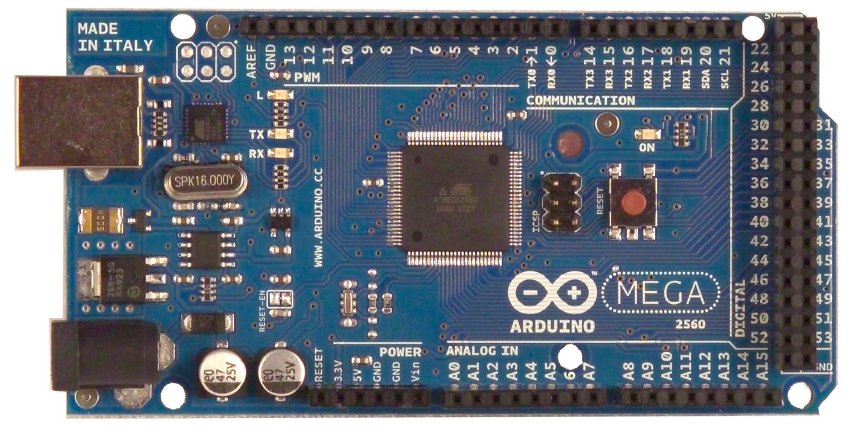
\includegraphics[width=0.99\textwidth]{graphics/MCU/arduino_mega.png}
\captionof{figure}{Arduino Mega Board \cite[S.1]{arduinoMega}}
\label{fig:arduinoMega}
\end{minipage}}

\begin{table}[h]
\centering
\caption{Technische Daten \cite[S.3]{arduinoMega}}
\begin{tabular}{|l|l|}
\hline 
Microcontroller & ATmega2560 \\ 
\hline 
Operating Voltage & 5V \\ 
\hline 
Digital I/O Pins & 54  \\ 
\hline 
Analog Input Pins & 16 \\ 
\hline 
Flash Memory & 256 KB, 8 KB werden vom bootloader benötigt\\ 
\hline 
SRAM & 8 KB \\ 
\hline 
EEPROM & 4 KB \\ 
\hline 
Clock Speed & 16 MHz \\ 
\hline 
\end{tabular}
\label{tab:arduinoMega_technischeDaten}
\end{table}
\newpage
\subsubsection{Ergänzungen aus der Bachelor-Thesis}
{\begin{minipage}[b][220pt][t]{0.55\textwidth}
Während der Bachelor-Thesis kam die Idee auf, eine kleinere MCU zu verwenden. Eine kleinere MCU hat die Vorteile, dass diese günstiger ist in der Anschaffung, einen geringeren Stromverbrauch aufweist und weniger Platz auf dem PCB benötigt.  Aufgrund der Firmware wird jedoch eine erhöhte Menge Speicher alloziert, weshalb die \textit{Data Memory Usage} des verwendeten ATMega328 zu klein war und wieder auf den bereits für das Prototyping verwendeten ATMega2560 zurückgegriffen werden musste. Für die Wetterstation wird schlussendlich kein Board mehr verwendet, sondern der Mikroprozessor (ATMega2560, siehe Abbildung \ref{fig:ATMega2560}) selbst auf dem PCB platziert. Damit dieser wie gewünscht funktioniert, werden weitere Bauteile verwendet. Im nächsten Abschnitt wird mehr auf die zusätzlichen Bauteile eingegangen.
\end{minipage}}
{\begin{minipage}[b][220pt][t]{0.44\textwidth}
\centering
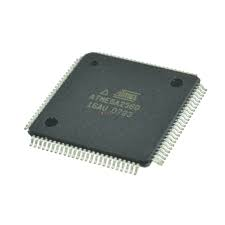
\includegraphics[width=0.8\linewidth]{graphics/MCU/ATMega2560.jpg}
\captionof{figure}{Der Mikroprozessor ATMega2560, ohne Board.}
\label{fig:ATMega2560}
\end{minipage}}

Wie in der Übersicht in Abbildung \ref{fig:Uebersicht_PCB_MCU_RTC_SD_Sense} zu sehen ist, wird für die MCU ein ICSP-Header (In Circuit System Programming) benötigt. Durch diesen ICSP-Header kann die Firmware über ein AVR-Dragon auf die MCU geladen werden, wobei spätere Anpassungen der Firmware möglich bleiben, was wiederum zur Skalierbarkeit (Erweiterbarkeit) des Systems beiträgt. Die MCU selbst (ATMega2560) hat einen internen Clock, welcher über ein RC-Oszillator generiert wird und eine wesentlich höhere Temperaturabhängigkeit besitzt als ein externer Quarz. Aus diesem Grund wird ein externer Quarz verwendet, wie in Abbildung \ref{fig:Uebersicht_PCB_MCU_RTC_SD_Sense} ebenfalls ersichtlich ist. Ausserdem werden Kondensatoren bei den 3.3V-Speisepins verwendet, um Induktivitäten durch Leiterbahnlängen auszugleichen. Um das System rebooten zu können wird ein Reset-Button hinzugefügt, wobei über eine Status-LED der Betrieb der MCU ersichtlich ist. Über ein CLI (Command Line Interface) soll mit der MCU interagiert werden können, wodurch eine Verbindung mit einem $\mu$USB-Interface erforderlich wird. Die Sensorik, die RTC (Real Time Clock) und die SIM808 werden ebenfalls mit der MCU verbunden, was die MCU zum Herzstück der Wetterstation macht, da hier alle Daten verarbeitet werden. Die verarbeiteten Daten werden in der angeschlossenen Datenspeicherung wiederum gespeichert.\\[0.5cm]
In diesem Kapitel wurde die Thematik der MCU eingehend thematisiert. RC-Oszillatoren und Quarze wurden ebenfalls erwähnt. Aus diesem Grund wird im nächsten Kapitel die RTC näher erläutert.
